\documentclass[12pt]{article}
%\usepackage[margin=1.25in]{geometry}                % See geometry.pdf to learn the layout 
\usepackage{graphicx}
\usepackage{amssymb}
\usepackage{epstopdf}
\usepackage{hyperref}
\usepackage{setspace}
\usepackage{natbib}
\usepackage{booktabs}
\usepackage{amsmath}
\usepackage{caption}

\begin{document}
\title{Inferring Unobserved Firm Networks}
\author{Jesse Tweedle}
\date{}
%\address{Statistics Canada\\University of Calgary}
%\email{jesse.tweedle@gmail.com}


 \maketitle

\begin{abstract}

Use data and machine learning to infer unobserved firm-firm trading networks. Given data on firm characteristics, and a detailed geographic trading network, infer the unobserved firm-firm trading network that matches the Canadian national accounts.

\end{abstract}

\section{Equations}

The first set of equations to match is 
\begin{gather}
\sum_{r=1}^R M_r a_{ri} + \sum_{j=1}^N (1-\beta_j) s_j g_{ji} = s_i , \quad i = 1,\ldots, N
\end{gather}
Which I rewrite as (and add important other restrictions)
\begin{gather}
\label{eq:mc}
M \cdot a_{\cdot i} + (1-\beta) s \cdot g_{\cdot i} = s_i, \quad i = 1,\ldots, N \\
a_{ri} \geq 0, \quad a_{ri} - 1 \leq 0 \\
g_{ij} \geq 0, \quad g_{ij} - 1\leq 0 \\
g_{ii} = 0 \\
\sum_{i \in N} a_{ri} = 1 \label{eq:rowsuma}\\
\sum_{j \in N} g_{ij} = 1\label{eq:rowsumg}
\end{gather}

\[
X_{mc} = 
\begin{bmatrix}
    M & (1-\beta) s &  0 & 0 & \dots  & 0 & 0\\
    0 & 0 & M & (1-\beta) s &\dots  & 0 & 0 \\
    \vdots & \vdots & \vdots & \vdots & \ddots & \vdots & \vdots  \\
    0 & 0 & 0 & 0 & \dots  & M & (1-\beta) s
\end{bmatrix}
\]

Then $X_mc$ has dimensions $N \times (R+N)N$ (this may be a problem later---it's sparse but still has exactly $(R+N)N$ non-zero entries, which is too many if $N$ is any economically reasonable number). $mc$ stands for market clearing, and represents Equation \eqref{eq:mc}.

There are also $R+N$ equations that require the expenditure shares add up to 1.

\[
X_{ag} = 
\begin{bmatrix}
    1 & 0 &\dots  & 0 & \dots & 1 & 0 & \dots & 0\\
    0 & 1 &\dots  & 0 & \dots & 0 & 1 &\dots  & 0\\
    \vdots & \vdots & \ddots & \vdots & \dots & \vdots & \vdots & \ddots & \vdots \\
    0 & 0 & \dots  & 1 & \dots & 0 & 0 &\dots  & 1
\end{bmatrix} = 
\underbrace{\begin{bmatrix}
I_{R+N} \ldots I_{R+N}
\end{bmatrix}}_{(R+N) \times (R+N) N}
\]

%And $X_g$ is similar,
%\[
%X_{g} = 
%\underbrace{\begin{bmatrix}
%I_N \ldots I_N
%\end{bmatrix}}_{N \times N^2}
%\]
%Combine those two into $Z$
%\[
%Z = 
%\begin{bmatrix}
%X_a & 0 \\
%0 & X_g
%\end{bmatrix}
%\]


And then construct $X$ as
\[
X = 
\begin{bmatrix}
X_{mc} \\
X_{ag}
\end{bmatrix}
\]

And 
\[
c = 
\begin{bmatrix}
s \\
1_R \\
1 -\beta \\
\end{bmatrix}
\]

Let $y$ be a combined vectorized $A$ and $G$, so that $y$ is a vector with length $(R + N) N$. 
\[ 
%y' = (a_{11},a_{21},\ldots,a_{R1},\ldots,a_{1N},\ldots,a_{RN},g_{11},g_{21},\ldots,g_{N1},g_{1N},\ldots,g_{NN}) 
y' = (a_{11},a_{21},\ldots,a_{R1},g_{11},g_{21},\ldots,g_{N1},\ldots,a_{1N},\ldots,a_{RN},g_{1N},\ldots,g_{NN}) 
\]
Or, write $a_{\cdot i}$ as the $i$-th column of $A$, and so on.
\[ 
%y' = (a_{\cdot 1},\ldots,a_{ \cdot N},g_{ \cdot 1},\ldots,g_{ \cdot N})
y' = (a_{\cdot 1},g_{ \cdot 1},\ldots,a_{ \cdot N},g_{ \cdot N})
\]

We have the three things we need: $c$ is $(N + R + N) \times 1$, $y$ is $(RN + N^2)\times 1$, and $X$ is $(N+R+N)\times (RN + N^2)$, and the set of equations to solve is:

\begin{gather}
X y = c
\end{gather}

%Or,
%\[
%\underbrace{\begin{bmatrix}
%    I & 0 &\dots  & 0 & s & 0 & \dots & 0\\
%    0 & I &\dots  & 0 & 0 & s &\dots  & 0\\
%    \vdots & \vdots & \ddots & \vdots & \vdots & \vdots & \ddots & \vdots \\
%    0 & 0 & \dots  & I & 0 & 0 &\dots  & s
%\end{bmatrix}}_{N \times (RN+N^2)}
%\underbrace{\begin{bmatrix}
%	a_{\cdot 1} \\
%	a_{\cdot N} \\
%	\vdots \\
%	g_{\cdot 1} \\
%	g_{\cdot N} 	
%\end{bmatrix}}_{(RN+N^2) \times 1}
%=
%\underbrace{\begin{bmatrix}
%	s_1 \\
%	\vdots \\
%	s_{N} 	
%\end{bmatrix}}_{N\times 1}
%\]

And the $\ell 1$ minimization problem is:
%Other characteristics are $c$, $N\times1$ (or more), and $X$, $N \times (RN + N^2)$. Then the problem is 
\begin{gather}
\min_y || X y - c||_2 + \lambda || y ||_{\ell 1}
\end{gather}

Or the elastic net:
\begin{gather}
\min_y || X y - c||_2 + \lambda \left( (1-\alpha) \frac{1}{2} || y ||^2_{\ell 2} + \alpha || y ||_{\ell 1} \right)
\end{gather}


This is an underdetermined system, since the number of variables is much more than the number of ``observations'' (which, in this case, are firm characteristics and later, national accounts). The estimated $y$ gives the most sparse implied network that matches the national accounts. Density can be increased by using elastic-net (which combines $\ell 1$ and $\ell 2$ regularization).  To use the geographic trade network, we assume the implied firm-firm network identified from that as a subset of the true network, and leave those edges out of the penalty $||y||$.

Now use \texttt{glmnet} to solve this problem. Simulation testing: set $R$, $N$, set , draw random $\beta_i$ and $s_i$, random firm locations $r_i$, calculate regional income $I_r = \sum_{i \in r} \beta_i s_i$, then construct $X$ and $c$, then run glmnet for different $R,N$, skewness in $s$ and so on. See if anything works.

\section{Add industry equations}

Each firm $i$ now has an industry $k$. 
%An industry intermediate IO table looks like
%\[
%G^I =
%\begin{bmatrix}
%    g^I_{11} & g^I_{12} &\dots  & g^I_{1K}  \\
%    g^I_{21} & g^I_{22}  &\dots  & g^I_{2K} \\
%    \vdots & \vdots & \ddots & \vdots \\
%    g^I_{K1} & g^I_{K2} & \dots  &  g^I_{KK}
%\end{bmatrix}
%\]

Which we can possibly get to via $G$ by...multiplying a firm-industry matrix $K$
\[
K = [x_{ik} ]
\]
where $x_{ik} = \mathbf{1} \{ \text{firm } i \in \text{industry } k \}$. This is a sparse matrix with one non-zero element per row, and $K$ is $N \times K$. 
%Then I can possibly get $G^I$ by
%\[
%G^I = IK' \times G \times IK
%\]
%Well, probably not, but something like that. Will probably have to go to actual expenditures, and then normalize, or something.

\begin{gather}
\sum_{j \in k'} \sum_{i \in k} (1-\beta_i) s_i g_{ij} = x_{kk'}
%g^I_{IJ} \sum_{i\in I} (1-\beta_i) s_i = \sum_{j \in J} \sum_{i \in I} (1-\beta_i) s_i g_{ij} \\
%s_I g^I_{IJ} = \sum_{j \in J} \sum_{i \in I} (1-\beta_i) s_i g_{ij} \\
%\sum_{j \in J} \sum_{i \in I} (1-\beta_i) s_i g_{ij} = s_I g^I_{IJ}
\end{gather}
 
 So some of these are non-zero. Maybe not many. But important bit is that they can go into the first stage. So there are $K^2$ equations here. They only use the parameters $g_{ij}$ (for now---final demand maybe comes later).
 
 Somehow need to multiply the $s_i$ by $g_{ij}$, then aggregate by industries. Which means I need to use $IK$. The left hand side needs to be a matrix that is $K^2 \times (R+N)N$, call it $X_{\text{ind}}$. One row $i'$ of $X_{\text{ind}}$ represents an industry pair $IJ$. It has non-zero entries $s_i$ when the column $j'$ of $X_{ind}$ matches an element of $y$. E.g., if the $j'$-th element of $y$ is $g_{ij}$, then $X_{\text{ind}}(i',j') = s_i$ if $i'=(k,k')$, $i \in k, j \in k'$. \emph{If} the firms are sorted by industries, it looks like

\[
X_{ind} =
\begin{bmatrix}
    0  & s &  0 & 0 &\dots  &  0 & 0 \\
    0 & 0  & 0 &  s & \dots  & 0 & 0 \\
    \vdots & \vdots & \ddots & \vdots \\
    0 & 0  & 0 & 0  & \dots  &  0 & s
\end{bmatrix}
\]

In the program / code, the idea is to take the a firm-firm matrix and reshape it using industry information into a matrix that is $K^2 \times (R+N)N$, where each row represents an industry pair. 

%First, for a given industry pair $(k,k')$, look at a firm $j$ in $k'$. 
Write a dataset where each observation has two firms $i$ and $j$, their indutries $k_i$ and $k_j$, and the input firm's expenditure $(1-\beta_i) s_i$.  For each producer $j$, convert this dataframe into a matrix with the following rule:

\begin{verbatim}
z_j <- with(q, sparseMatrix(i=((ki-1)*K+kj),j=i,x=x,dims=c(K^2,N)))
\end{verbatim}

Then the full matrix is
\[
X_{ind} =
\begin{bmatrix}
    0  & z_1 &  0 & z_2 &\dots  &  0 & z_N 
\end{bmatrix}
\]
where the 0s are $K^2 \times R$ zero matrices, which will be replaced later when I add in regional final demand expenditures by industry (if I can work that out). Each $z_j$ is $K^2 \times N$, which makes the whole thing $K^2 \times (R+N)N$. Write the RHS of this equation as

\[
c_{ind} = ( x_{11} , x_{12} , \dots , x_{1K}, x_{21}, \dots, x_{KK} )
\]

\[
X = 
\begin{bmatrix}
X_{mc} \\
X_{ag} \\
X_{ind}
\end{bmatrix}
\]

And 
\[
c = 
\begin{bmatrix}
s \\
1_R \\
1 -\beta \\
c_{ind}
\end{bmatrix}
\]

\section{Extra details}
Since it's matching levels, it's more likely to get the equations with large RHS values correct. E.g., $s$ instead of $1_R$. But it depends on scaling. So, it works better if I use $M$ instead of $1_R$, and $(1-\beta)s$ instead of $(1-\beta)$. In addition, I can rescale the importance of certain equations by using penalties that depend on $M$ and $s$.

\section{Evaluation}

How well does it match the equations? I can graph the 

% Table created by stargazer v.5.2 by Marek Hlavac, Harvard University. E-mail: hlavac at fas.harvard.edu
% Date and time: Sun, Nov 06, 2016 - 20:11:38
% Requires LaTeX packages: dcolumn 
% Table created by stargazer v.5.2 by Marek Hlavac, Harvard University. E-mail: hlavac at fas.harvard.edu
% Date and time: Sun, Nov 06, 2016 - 20:22:54
\begin{table}[htbp!] 
\centering 
\footnotesize
  \caption{Evaluating the solution} 
  \label{}
\begin{tabular}{l rrrrr} 
\vspace{-4ex} \\
\toprule
% & \multicolumn{5}{c}{\textit{Dependent variable:}} \\ 
%\cmidrule{2-6} 
& \multicolumn{5}{c}{Actual equation value} \\ 
& All & $mc$ & $a$ & $g$ & $ind$ \\ 
\midrule
 Predicted eq. value & 1.000$^{***}$ & 1.000$^{***}$ & 1.000$^{***}$ & 1.001$^{***}$ & 1.010$^{***}$ \\ 
  & (0.0003) & (0.00000) & (0.000) & (0.003) & (0.004) \\ 
  & & & & & \\ 
 Constant & $-$0.0004 & $-$0.0003$^{***}$ & 0.0003$^{***}$ & $-$0.001 & $-$0.052$^{***}$ \\ 
  & (0.001) & (0.00000) & (0.00000) & (0.002) & (0.019) \\ 
\midrule
Observations & 2,120 & 1,000 & 20 & 1,000 & 100 \\ 
R$^{2}$ & 1.000 & 1.000 & 1.000 & 0.990 & 0.999 \\ 
%Adjusted R$^{2}$ & 1.000 & 1.000 & 1.000 & 0.990 & 0.999 \\ 
%Residual Std. Error & 0.032 (df = 2118) & 0.00000 (df = 998) & 0.00000 (df = 18) & 0.044 (df = 998) & 0.044 (df = 98) \\ 
\bottomrule
%\textit{Note:}  & \multicolumn{5}{r}{$^{*}$p$<$0.1; $^{**}$p$<$0.05; $^{***}$p$<$0.01} \\ 
\end{tabular} 
\end{table} 

What do the plots look like? Also have sensitivity, specificity, and positive predictive value. And then rowsums of $\hat{A}$ and $\hat{G}$.

\begin{figure}
  \caption{Predicted expenditure share vs. firm size}
  \centering
	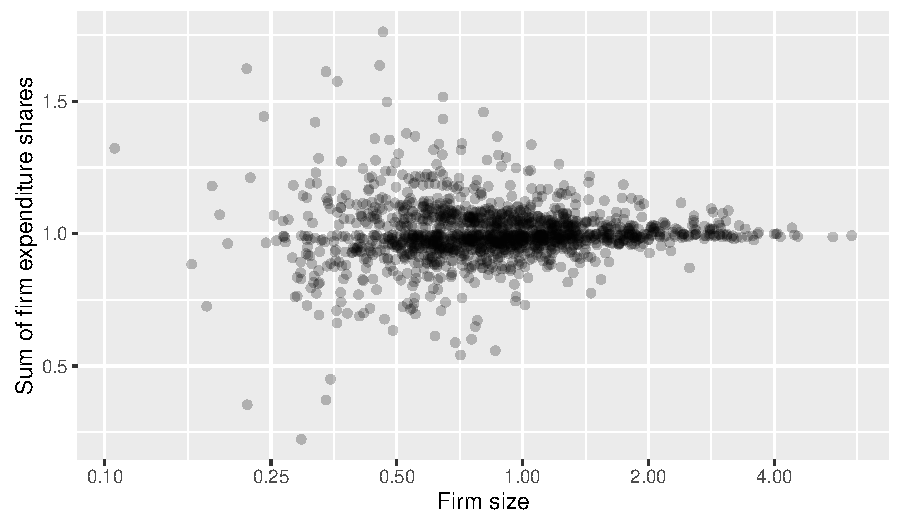
\includegraphics[width=\textwidth]{../assets/shares-v-size}
	\caption*{\small \emph{Notes:} all of the firm expenditure shares should be equal to 1. Most are $1\pm0.05$, and it gets more accurate for larger firms.}
\end{figure}

\bibliographystyle{chicago}
\bibliography{inferring-firm-networks-2}

\end{document}








